\section{Methodology}
\label{sec:method}

\begin{figure*}[t]
    \centering
    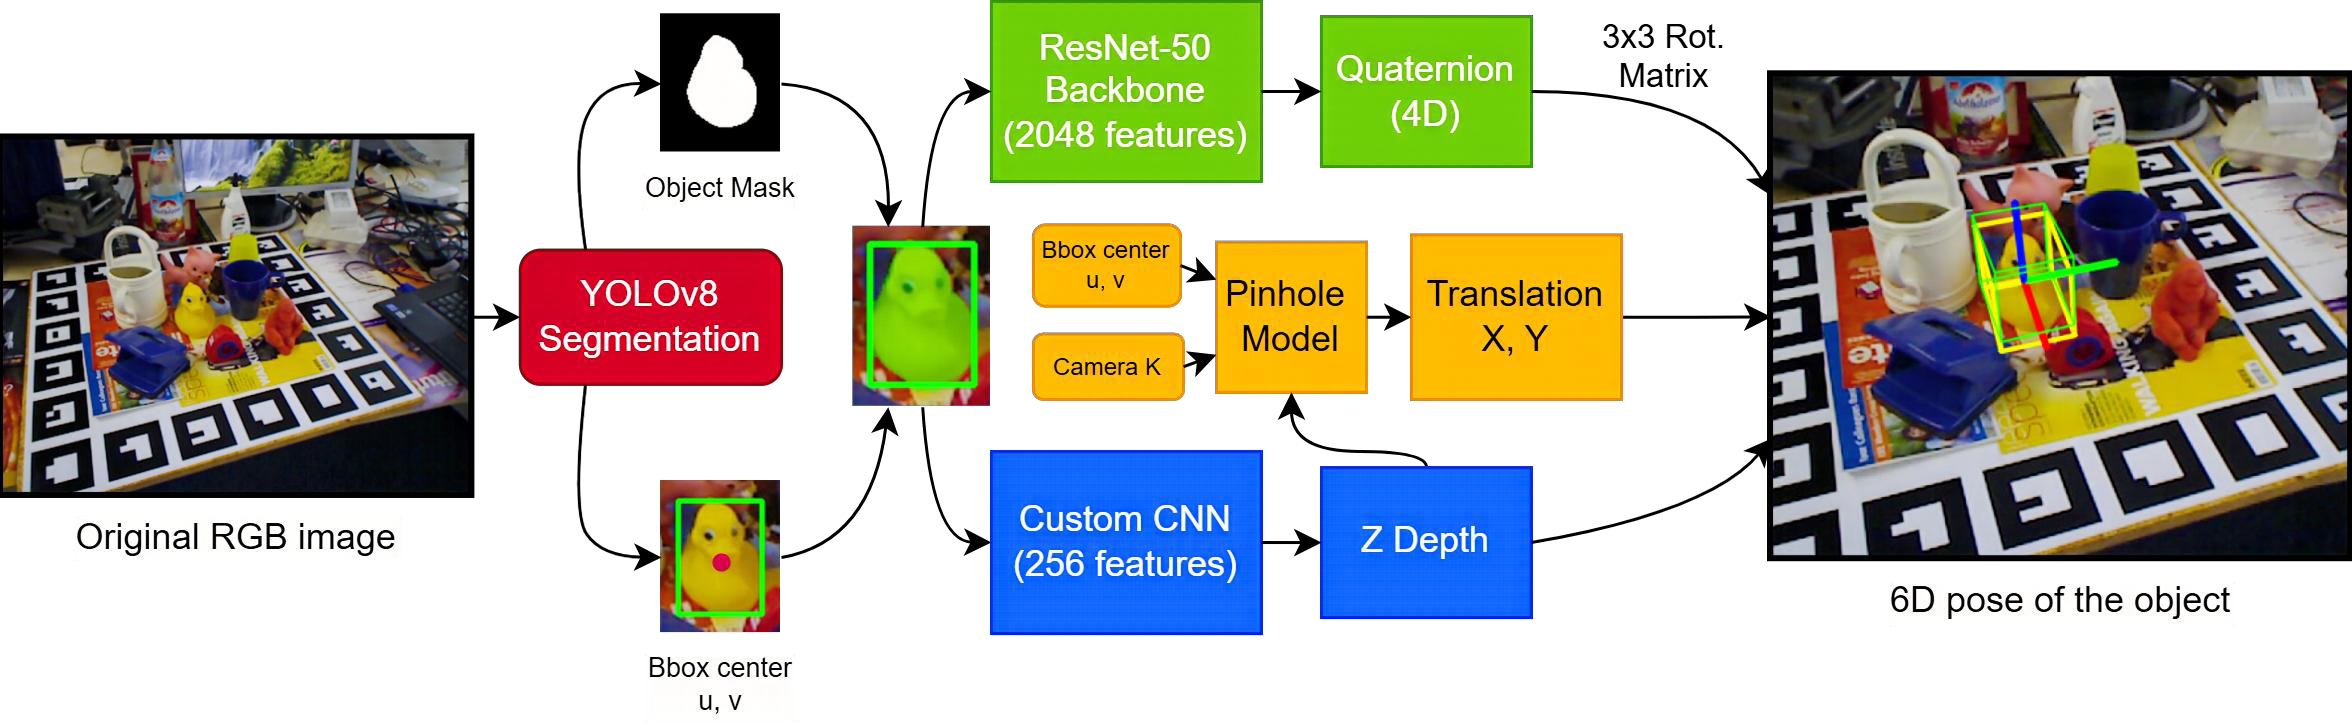
\includegraphics[width=\textwidth]{sec/figures/rgb-pipeline.png}
    \caption{RGB model pipeline.}
    \label{fig:rgb_pipeline}
\end{figure*}

\paragraph{Overview.}
Our pipeline consists of two stages: (1) object detection and segmentation using YOLOv8, and (2) pose estimation using either an RGB-only or RGB-D model. Both models predict rotation as a quaternion and leverage geometric constraints from the pinhole camera model to derive translation.

\paragraph{Object Detection.}
We use YOLOv8n-seg~\cite{yolov8} fine-tuned on LineMOD, which outputs bounding boxes, instance segmentation masks, and class labels for each detected object.

\subsection{RGB Model}

The RGB model pipeline is shown in \cref{fig:rgb_pipeline}. From each detection, we extract a 224×224 crop with 1.2× padding, concatenated with the binary mask to form a 4-channel input. RGB channels are normalized using ImageNet statistics.

\subsubsection{Two-Stream Architecture}
\begin{table}[h]
\centering
\caption{RGB Model Architecture (26.6M params)}
\label{tab:rgb_arch}
\scriptsize
\begin{tabular}{l|c|c}
\toprule
\textbf{Layer} & \textbf{Config} & \textbf{Output} \\
\midrule
\multicolumn{3}{c}{\textit{Rotation Stream (ResNet-50)}} \\
\midrule
Conv1 & 4$\to$64, 7$\times$7, s2 & 64$\times$112 \\
Layer1-4 & Standard ResNet-50 & 2048 \\
\midrule
\multicolumn{3}{c}{\textit{Rotation Head}} \\
\midrule
FC & 2048$\to$1024$\to$512$\to$4, L2-norm & 4 \\
\midrule
\multicolumn{3}{c}{\textit{Depth Stream (CNN)}} \\
\midrule
Conv1-4 & 4$\to$32$\to$64$\to$128$\to$256 & 256 \\
\midrule
\multicolumn{3}{c}{\textit{Z-Depth Head}} \\
\midrule
FC & 256$\to$128$\to$64$\to$1, Sigmoid & 1 \\
\bottomrule
\end{tabular}
\end{table}

The model employs two parallel streams (\cref{tab:rgb_arch}):

\textbf{Rotation Stream:} A modified ResNet-50 backbone with the first conv layer adapted to accept 4 channels (RGB weights from ImageNet, mask channel initialized with small random values). The backbone outputs 2048-D features feeding a rotation head that produces a unit quaternion.

\textbf{Depth Stream:} A lightweight CNN produces 256-D features, feeding a depth head that outputs Z-depth scaled to [0.3, 1.7]m (determined by analyzing LineMOD ground truth depths: 0.51-1.45m).



\subsubsection{Geometric Translation}
X and Y translation are derived analytically using the pinhole camera model:
\begin{equation}
    t_x = \frac{(u - c_x) \cdot t_z}{f_x}, \quad t_y = \frac{(v - c_y) \cdot t_z}{f_y}
\end{equation}
where $(u, v)$ is the bounding box center, $t_z$ is predicted depth, and $(f_x, f_y, c_x, c_y)$ are camera intrinsics. This reduces the learning problem to rotation and depth only.

\begin{figure*}[t]
    \centering
    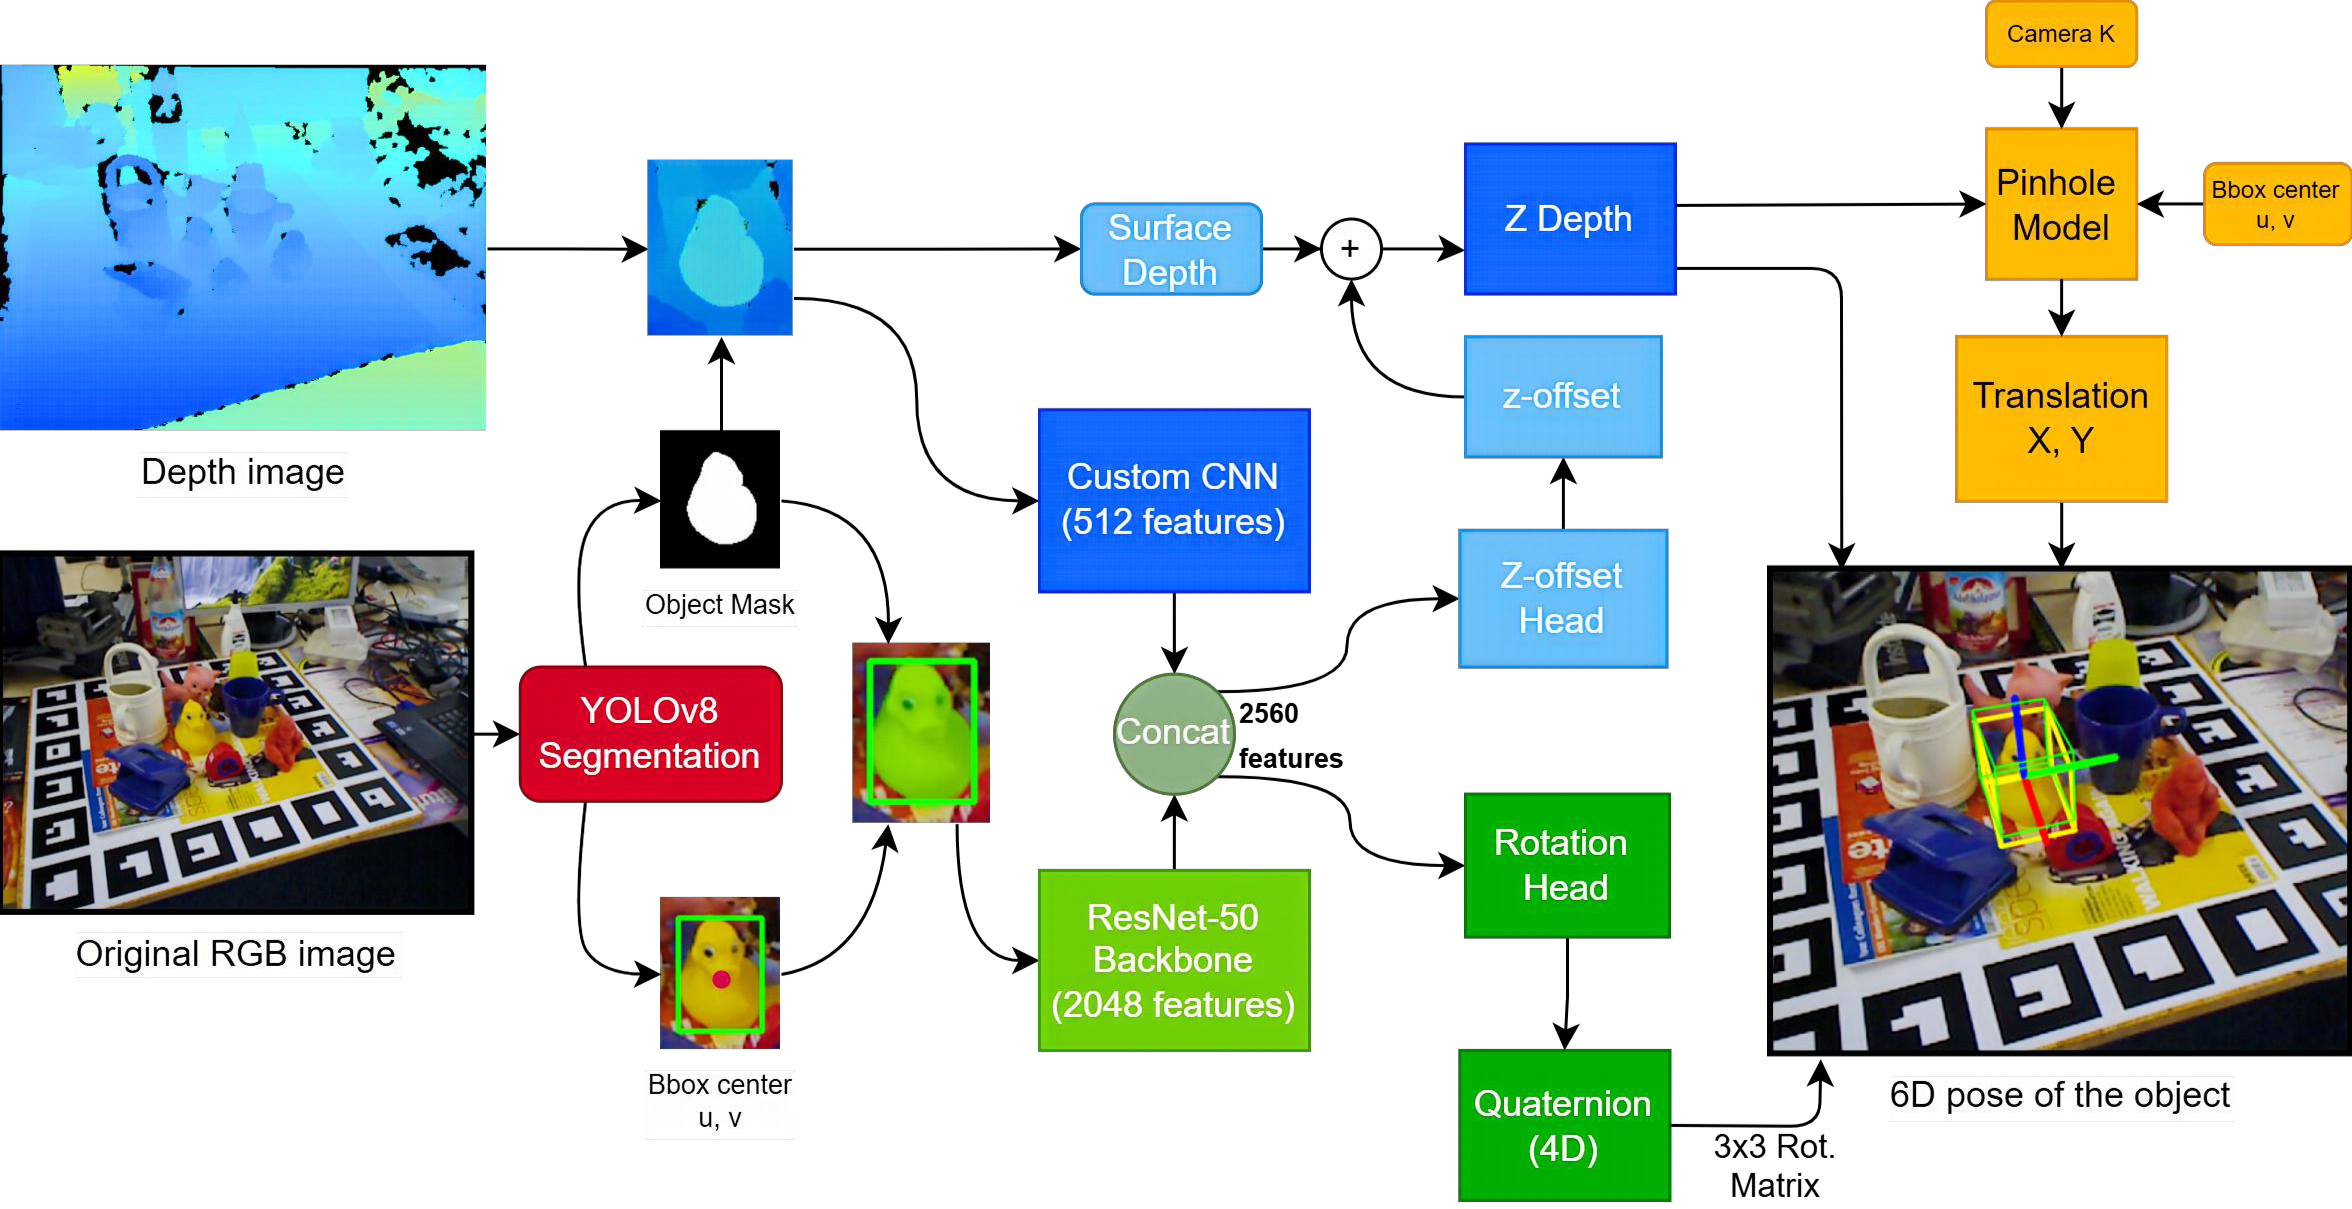
\includegraphics[width=\textwidth]{sec/figures/rgbd-pipeline.png}
    \caption{RGB-D model architecture.}
    \label{fig:rgbd_pipeline}
\end{figure*}

\subsection{RGB-D Model}

The RGB-D model (\cref{fig:rgbd_pipeline}) extends the RGB model with depth information, forming a 5-channel input (RGB + Depth + Mask). The depth channel is preprocessed with bilateral filtering and normalized to [0, 1].

\subsubsection{Dual-Stream Fusion}
The 5-channel input is split into two streams (\cref{tab:rgbd_arch}):

\textbf{RGB+Mask Stream (4ch):} ResNet-50 backbone producing 2048-D features.

\textbf{Depth+Mask Stream (2ch):} Custom CNN producing 512-D features.

Features are concatenated (2560-D) and fed to rotation and z-offset heads.

\begin{table}[h]
\centering
\caption{RGB-D Model Architecture (29.7M params)}
\label{tab:rgbd_arch}
\scriptsize
\begin{tabular}{l|c|c}
\toprule
\textbf{Layer} & \textbf{Config} & \textbf{Output} \\
\midrule
\multicolumn{3}{c}{\textit{RGB+Mask Stream (ResNet-50)}} \\
\midrule
Conv1, Layer1-4 & Same as RGB model & 2048 \\
\midrule
\multicolumn{3}{c}{\textit{Depth+Mask Stream (CNN)}} \\
\midrule
Conv1-4 & 2$\to$64$\to$128$\to$256$\to$512 & 512 \\
\midrule
\multicolumn{3}{c}{\textit{Feature Fusion + Heads}} \\
\midrule
Concat & [RGB; Depth] & 2560 \\
Rotation Head & 2560$\to$1024$\to$512$\to$4 & 4 \\
Z-Offset Head & 2560$\to$512$\to$128$\to$1 & 1 \\
\bottomrule
\end{tabular}
\end{table}

\subsubsection{Z-Offset Formulation}
Instead of predicting absolute depth, the RGB-D model predicts a small offset from the sensor measurement: z\_final = z\_sensor + z\_offset. The sensor depth (median of masked pixels) represents the visible surface; the network learns to adjust this to the object center (typically ±20-50mm).

\textbf{Benefits:} (1) Simpler learning target (small corrections vs absolute depth), (2) leverages accurate sensor measurements as prior, (3) better initialization (z\_offset=0 gives reasonable estimate).

X and Y translations use the same geometric formulation as the RGB model.